\chapter{Time Systems and the Rotating Earth}

\section{Introduction: The Duality of Time and Position in Astronomy}

Every observational measurement in astronomy is fundamentally intertwined with the concept of time. When an astronomer points a telescope toward a distant nebula, calculates the ephemeris of a planet, or measures the pulse arrival times from a millisecond pulsar, time acts simultaneously as an independent physical coordinate and as a geometric bridge between reference frames.

In terrestrial physics, time is measured by a clock at rest in a laboratory. In observational astrophysics, however, our primary observatory is a non-inertial platform --- the spinning, orbiting, and precessing Earth. Because the Earth rotates eastward about its axis, the entire celestial sphere appears to revolve westward. Consequently, \textbf{an angle of time is directly equivalent to an angle of celestial position}:
\begin{equation}
	1^{\rm h} \equiv 15^\circ, \qquad 1^{\rm m} \equiv 15' = 0.25^\circ, \qquad 1^{\rm s} \equiv 15'' = 0.004167^\circ.
	\label{eq:time_angle_conversion}
\end{equation}
Before establishing spatial coordinate grids on the sky (the subject of Chapter~2), we must construct the temporal frameworks that govern them. This chapter develops astronomical timekeeping from first principles:
\begin{enumerate}[leftmargin=1.5em, itemsep=0.3em]
	\item \textbf{Rotational Clocks:} The fundamental beat between the Earth's daily spin and its annual orbital revolution (solar vs. sidereal days).
	\item \textbf{Local and Global Topocentric Time:} How terrestrial longitude establishes Local Sidereal Time ($\LST$) and links local horizons to the stars.
	\item \textbf{Orbital Non-Uniformities:} The physical origins of the Equation of Time ($\EoT$) and the seasonal migration of the Sun.
	\item \textbf{Gyroscopic Dynamics:} The physical consequences of lunisolar precession and nutation on reference epochs.
	\item \textbf{Modern Relativistic Time Scales:} The progression from Earth rotation ($\UT1$) to atomic standards ($\TAI, \UTC$) and relativistic coordinate time ($\TT, \TDB$).
	\item \textbf{Continuous Chronology:} The Julian Date system ($\JD, \MJD$) used in computational ephemerides.
\end{enumerate}

\section{Two Natural Clocks: The Solar Day and the Sidereal Day}

Every classical timekeeping system is anchored to the Earth's rotation. However, because rotation must be measured relative to a chosen reference direction, nature presents two fundamentally distinct clocks.

\begin{definition}[Solar Day]
	The \emph{solar day} is the time interval between two successive meridian transits of the Sun (successive local solar noons). The civil calendar defines the \emph{mean solar day} to be exactly $24^{\rm h} = 1440^{\rm m} = 86{,}400\,\mathrm{s}$.
\end{definition}

\begin{definition}[Sidereal Day]
	The \emph{sidereal day} is the time interval between two successive meridian transits of the vernal equinox $\hat\gamma$ (or equivalently, a fixed direction toward the distant inertial background of stars). Its physical duration is
	\begin{equation}
		T_{\rm sid} \simeq 23^{\rm h}56^{\rm m}04.0905^{\rm s} \approx 86{,}164.0905\,\mathrm{s}.
		\label{eq:sidereal_day_length}
	\end{equation}
\end{definition}

\subsection{Physical Origin of the Four-Minute Difference}

Why is the solar day approximately $3^{\rm m}56^{\rm s}$ longer than the sidereal day?

\begin{figure}[htbp]
	\centering
	\begin{tikzpicture}[>=Stealth, font=\sffamily, scale=1.3]
		\coordinate (Sun) at (-1.5, 0);
		\coordinate (Earth1) at (6.5, 0);
		\coordinate (Earth2) at (5.0532, 4.5886);
		\draw[line width=1.2pt] (Sun) -- (Earth1);
		\draw[line width=1.2pt] (Sun) -- (Earth2);
		\draw[line width=1.5pt, ->] (Sun) ++(-5:8.0) arc[start angle=-5, end angle=50, radius=8.0];
		\node[font=\large, anchor=south west] at (4.2, 6.4) {Orbit around Sun (counter-clockwise)};
		\draw[fill=yellow, line width=1.2pt] (Sun) circle (0.75);
		\node[font=\bfseries\large] at (Sun) {Sun};
		\draw[dashed, ->, line width=1.2pt] (-2.25, 0) -- (-3.8, 0);
		\shade[ball color=cyan!60!blue!40] (Earth1) circle (0.85);
		\draw[line width=1.2pt] (Earth1) circle (0.85);
		\node[font=\bfseries\large] at (Earth1) {Earth};
		\node[font=\bfseries\large, anchor=south west] at (6.8, 0.8) {Day 1 (Noon)};
		\draw[line width=1.2pt] (6.5, -0.85) -- (6.5, -1.45);
		\shade[ball color=cyan!60!blue!40] (Earth2) circle (0.85);
		\draw[line width=1.2pt] (Earth2) circle (0.85);
		\node[font=\bfseries\large, anchor=south west] at (5.3, 5.4) {Day 2 (Noon)};
		\draw[fill=cyan!80!black!30, line width=0.8pt] (Earth2) circle (0.5);
		\draw[->, line width=1.2pt] (Earth2) ++(0:0.4) arc[start angle=0, end angle=230, radius=0.4];
		\draw[dashed, ->, line width=1.2pt] (Earth2) ++(-0.85, 0) -- (-3.2, 4.5886);
		\node[align=center, font=\large, anchor=south] at (-0.8, 4.65) {Inertial reference direction\\(defines sidereal day)};
		\draw[line width=1pt] (Sun) ++(1.8, 0) arc[start angle=0, end angle=35, radius=1.8];
		\node[font=\large, anchor=west] at (0.8, 0.5) {$\Delta\theta_{\rm orb} \approx \frac{360^\circ}{365.2422\text{ d}} \approx 0.9856^\circ/\text{day}$};
		\draw[<->, line width=1.2pt] (Earth2) ++(180:1.7) arc[start angle=180, end angle=215, radius=1.7];
		\node[align=center, font=\large, anchor=east] at (3.0, 3.6) {Spinning Earth must rotate an extra\\$\sim 0.9856^\circ$ ($\approx 3^{\rm m}56^{\rm s}$) to face Sun};
	\end{tikzpicture}
	\caption{Geometric relationship between the sidereal day and the solar day. Because the Earth revolves around the Sun in the same direction that it spins (prograde rotation), one true $360^\circ$ rotation relative to the stars leaves the observer short of facing the Sun by the orbital angle $\Delta\theta_{\rm orb}$.}
	\label{fig:orbit-sidereal}
\end{figure}

As shown in Figure~\ref{fig:orbit-sidereal}, the Earth revolves along its orbit in the same counter-clockwise direction (viewed from the North Celestial Pole) as its axial spin. During the time required for one full $360^\circ$ rotation relative to the stars (one sidereal day), the Earth advances along its orbit by:
\begin{equation}
	\Delta\theta_{\rm orb} = \frac{360^\circ}{365.2422\ \text{days}} \approx 0.985647^\circ/\text{day} \approx 1^\circ/\text{day}.
\end{equation}
To bring the Sun back onto the observer's local celestial meridian, the Earth must rotate through an additional angle equal to $\Delta\theta_{\rm orb}$.

Because the Earth completes a full $360^\circ$ rotation in $24^{\rm h} = 1440^{\rm m}$, the rotational conversion rate is:
\begin{equation}
	\frac{1440^{\rm m}}{360^\circ} = 4^{\rm m}/\text{degree}.
\end{equation}
The additional time required is therefore:
\begin{equation}
	\Delta t = 0.985647^\circ \times 4^{\rm m}/^\circ = 3.942588^{\rm m} \approx 3^{\rm m}56.55^{\rm s}.
\end{equation}

\subsection{Frequency Beat Derivation}

We can formulate this relationship with mathematical elegance in the frequency domain. Let $\omega_{\rm sidereal} = 2\pi/T_{\rm sid}$ be the Earth's inertial spin angular velocity, and let $\Omega_{\rm orb} = 2\pi/T_{\rm orb}$ be the mean orbital angular velocity of the Earth around the Sun ($T_{\rm orb} = 1\ \text{tropical year} = 365.2422\ \text{solar days}$).

The apparent rotation frequency of the Sun in the observer's co-rotating frame is the beat frequency:
\begin{equation}
	\omega_{\rm solar} = \omega_{\rm sidereal} - \Omega_{\rm orb}.
	\label{eq:frequency_beat}
\end{equation}
Dividing by $2\pi$:
\begin{equation}
	\frac{1}{T_{\rm solar}} = \frac{1}{T_{\rm sidereal}} - \frac{1}{T_{\rm orb}}.
	\label{eq:period_beat_formula}
\end{equation}
Multiplying through by $T_{\rm orb}$ (the number of days in one year):
\begin{keyresult}
	\begin{equation}
		N_{\rm sidereal} = N_{\rm solar} + 1 = 365.2422 + 1 = 366.2422\ \text{sidereal days/year}.
		\label{eq:sidereal_solar_relation}
	\end{equation}
\end{keyresult}
Over one complete orbital revolution, the Earth performs exactly \textbf{one more rotation relative to the universe than it does relative to the Sun}.

\paragraph{Observational Consequence:}
Because sidereal time gains $\approx 3^{\rm m}56^{\rm s}$ every solar day ($2^{\rm h}$ per month, $24^{\rm h}$ per year), a star that culminates at midnight on October 1 will culminate at 10:00 PM on November 1, and at midday (invisible in daylight) on April 1. This steady drift governs the seasonal visibility of constellations.

\section{The Three Astronomical Years: Tropical, Sidereal, and Anomalistic}

Just as there are two natural days, the Earth's complex orbital motion gives rise to three distinct definitions of a ``year'':

\begin{table}[htbp]
	\centering
	\begin{tabular}{@{}l p{6.8cm} l l@{}}
		\toprule
		\textbf{Year Type} & \textbf{Physical Definition} & \textbf{Duration (Days)} & \textbf{Difference from Tropical} \\
		\midrule
		\textbf{Tropical Year} & Equinox to equinox (cycle of the seasons) & $365.242190\ \text{d}$ & Baseline ($0^{\rm s}$) \\
		\textbf{Sidereal Year} & Orbit relative to distant fixed stars & $365.256363\ \text{d}$ & $+20^{\rm m}24.5^{\rm s}$ \\
		\textbf{Anomalistic Year} & Perihelion to perihelion transit & $365.259636\ \text{d}$ & $+25^{\rm m}07.5^{\rm s}$ \\
		\bottomrule
	\end{tabular}
	\caption{Comparison of the three primary astronomical years.}
	\label{tab:astronomical_years}
\end{table}

\begin{enumerate}
	\item \textbf{The Tropical Year ($365.242190\ \text{d}$):} The interval between successive passages of the Sun through the vernal equinox $\hat\gamma$. Because precession shifts the equinox westward by $50.29''/\text{yr}$ along the ecliptic, the Sun meets the equinox slightly before completing a full $360^\circ$ orbital circuit. The tropical year governs the calendar and the terrestrial cycle of seasons.
	\item \textbf{The Sidereal Year ($365.256363\ \text{d}$):} The true geometric period of one complete $360^\circ$ revolution of the Earth around the Sun relative to inertial space. It is longer than the tropical year by:
	\begin{equation}
		\Delta T_{\rm prec} \approx \frac{50.29''}{360^\circ \times 3600''/^\circ} \times 365.256\ \text{d} \approx 20.4\ \text{minutes}.
	\end{equation}
	\item \textbf{The Anomalistic Year ($365.259636\ \text{d}$):} The time between consecutive perihelion passages. Gravitational perturbations from other planets (principally Jupiter and Venus) cause the Earth's orbital major axis to precess prograde (eastward) by $\approx 11.6''/\text{year}$, making the anomalistic year $\approx 4.7\ \text{minutes}$ longer than the sidereal year.
\end{enumerate}

\paragraph{The Gregorian Calendar Reform.}
The Julian calendar assumed a year length of exactly $365.25\ \text{days}$, exceeding the tropical year ($365.2422\ \text{d}$) by $\approx 11.2\ \text{minutes/year}$ ($\approx 1\ \text{day}$ every 128 years). By 1582, the equinox had drifted from March 21 to March 11. Pope Gregory XIII introduced the modern rule: years divisible by 4 are leap years, \emph{except} century years not divisible by 400 (e.g., 1600 and 2000 were leap years, but 1700, 1800, 1900, 2100 are common years). This sets the average Gregorian calendar year to $365 + 97/400 = 365.2425\ \text{days}$, matching the tropical year to within 1 day in 3300 years.

\section{Longitude and Local Solar Time}

Because the Earth is a rigid body rotating with uniform angular velocity $\omega_\oplus = 15^\circ/\text{hour}$, all meridians sweep past the Sun simultaneously at the rate:
\begin{equation}
	\omega_\oplus = \frac{360^\circ}{24^{\rm h}} = 15^\circ/\text{hour} = 1^\circ/4^{\rm m} = 1'/4^{\rm s}.
\end{equation}
Two observers at longitudes $\lambda_1$ and $\lambda_2$ (measured East-positive from the Greenwich Prime Meridian) experience local solar noon at different Universal Times, offset by:
\begin{equation}
	\Delta t = \frac{\lambda_1 - \lambda_2}{\omega_\oplus}.
\end{equation}
The observer further east sees the Sun culminate earlier.

\paragraph{Civil Standard Time vs. Local Apparent Solar Time.}
Civil life cannot operate on continuous local solar time across adjacent cities. Instead, standard time zones are referenced to the local solar time of a designated reference meridian ($\lambda_{\rm ref}$).
\begin{keyresult}
	\begin{equation}
		\text{Local Solar Time} = \text{Civil Standard Time} - \frac{\lambda_{\rm ref} - \lambda_{\rm obs}}{\omega_\oplus}\quad (\text{if observer is west of ref. meridian}).
		\label{eq:civil_to_solar_time}
	\end{equation}
\end{keyresult}

\begin{example}[Local Solar Time at IISER Thiruvananthapuram]
	IISER TVM is located at longitude $\lambda_{\rm TVM} = 77.1382^\circ\text{E}$, west of the Indian Standard Time (IST) standard meridian $\lambda_{\rm IST} = 82.5^\circ\text{E}$.
	The longitude offset is:
	\[
	\Delta\lambda = 82.5^\circ - 77.1382^\circ = 5.3618^\circ.
	\]
	Converting to time:
	\[
	\Delta t = 5.3618^\circ \times 4\ \text{min}/^\circ = 21.4472\ \text{min} = 21^{\rm m}26.83^{\rm s}.
	\]
	When the civil clock reads exactly 12:00:00 IST, the local apparent solar time at IISER TVM is:
	\[
	\text{LST}_\odot = 12{:}00{:}00 - 0{:}21{:}27 = 11{:}38{:}33\ \text{AM}.
	\]
	Local solar noon at IISER TVM occurs at 12:21:27 IST.
\end{example}

\section{Local Sidereal Time (LST) and Greenwich Sidereal Time (GST)}

While solar time tracks the day-night cycle, telescopes must track stars across the sky. Astronomers therefore define a sidereal clock tied to the celestial sphere.

\begin{definition}[Local Sidereal Time]
	The \emph{Local Sidereal Time} ($\LST$) is defined as the right ascension currently crossing the observer's local celestial meridian:
	\begin{equation}
		\LST \equiv \alpha_{\rm Meridian}.
		\label{eq:lst_def}
	\end{equation}
\end{definition}

Because right ascension ($\alpha$) is measured eastward along the celestial equator from the vernal equinox $\hat\gamma$, and terrestrial longitude ($\lambda$) is measured eastward from Greenwich, $\LST$ is related to Greenwich Sidereal Time ($\GST$) by:
\begin{keyresult}
	\begin{equation}
		\LST = \GST + \lambda,
		\label{eq:lst_gst_relation}
	\end{equation}
\end{keyresult}
where longitude $\lambda$ is converted to time units ($15^\circ = 1^{\rm h}$).

\subsection{The Hour Angle ($H$)}

The \emph{Hour Angle} $H$ of a celestial object with cataloged right ascension $\alpha$ measures the time elapsed since the object crossed the local meridian:
\begin{keyresult}
	\begin{equation}
		H \equiv \LST - \alpha.
		\label{eq:hour_angle_def}
	\end{equation}
\end{keyresult}
\begin{itemize}
	\item $H = 0^{\rm h}$: The object is on the meridian (culmination / transit).
	\item $H > 0$: The object has passed the meridian and is moving toward the western horizon.
	\item $H < 0$: The object is in the eastern sky, approaching the meridian.
\end{itemize}

\section{The Sun's Coordinates and Ecliptic Motion Across the Seasons}

Because the Earth orbits the Sun in a plane tilted by the \emph{obliquity of the ecliptic} ($\epsilon \approx 23.44^\circ$) relative to the celestial equator, the Sun's apparent equatorial coordinates $(\alpha_\odot, \delta_\odot)$ change continuously throughout the year.

\begin{figure}[htbp]
	\centering
	\begin{minipage}[t]{0.48\textwidth}
		\centering
		
\includegraphics[width=\linewidth]{VERNAL_EQUINOX.png}
		\caption{The Sun crosses the celestial equator at the equinoxes ($\delta_\odot = 0^\circ$) and reaches extrema at the solstices ($\delta_\odot = \pm 23.44^\circ$).}
		\label{fig:vernal_equinox_fig}
	\end{minipage}
	\hfill
	\begin{minipage}[t]{0.48\textwidth}
		\centering
		
\includegraphics[width=\linewidth]{equinox_solstice_sm.png}
		\caption{Apparent path of the Sun along the ecliptic and the four cardinal seasonal milestones.}
		\label{fig:equinox_solstice_fig}
	\end{minipage}
\end{figure}

The Sun's equatorial coordinates and the corresponding Greenwich Sidereal Time at Greenwich solar noon ($\alpha_{\rm GM}$) at the cardinal seasonal milestones are:
\begin{align}
	\text{March (Vernal) Equinox (approx. Mar 21):}\quad &\alpha_\odot = 0^{\rm h}, &&\delta_\odot = 0^\circ, &&\alpha_{\rm GM} = 0^{\rm h}, \\
	\text{June (Summer) Solstice (approx. Jun 21):}\quad &\alpha_\odot = 6^{\rm h}, &&\delta_\odot \simeq +23.44^\circ, &&\alpha_{\rm GM} = 6^{\rm h}, \\
	\text{September (Autumnal) Equinox (approx. Sep 23):}\quad &\alpha_\odot = 12^{\rm h}, &&\delta_\odot = 0^\circ, &&\alpha_{\rm GM} = 12^{\rm h}, \\
	\text{December (Winter) Solstice (approx. Dec 21):}\quad &\alpha_\odot = 18^{\rm h}, &&\delta_\odot \simeq -23.44^\circ, &&\alpha_{\rm GM} = 18^{\rm h}.
\end{align}
At Greenwich local solar noon, the Sun is on the Greenwich meridian, so $\GST = \alpha_\odot$.

\section{The Equation of Time and the Solar Analemma}

A sundial measures \emph{Apparent Solar Time} ($\mathrm{AST}$), which tracks the hour angle of the physical Sun. However, apparent solar days are not of equal length throughout the year. Civil timekeeping is therefore based on \emph{Mean Solar Time} ($\mathrm{MST}$), which tracks a fictitious ``mean Sun'' that moves at a constant speed along the celestial equator.

\begin{definition}[Equation of Time]
	The \emph{Equation of Time} ($\EoT$) is defined as:
	\begin{keyresult}
		\begin{equation}
			\EoT \equiv \mathrm{AST} - \mathrm{MST} = \alpha_{\rm mean\,\odot} - \alpha_{\rm apparent\,\odot}.
			\label{eq:eot_def}
		\end{equation}
	\end{keyresult}
\end{definition}

The Equation of Time is the superposition of two independent physical phenomena:

\begin{enumerate}
	\item \textbf{Orbital Eccentricity Component ($e = 0.0167$):} In accordance with Kepler's Second Law, the Earth moves faster at perihelion (early January) and slower at aphelion (early July). The true Sun's apparent angular rate along the ecliptic varies as $\dot\lambda_\odot \propto 1/r^2$. This contributes an annual sinusoidal oscillation with an amplitude of $\approx 7.7\ \text{minutes}$:
	\begin{equation}
		\Delta t_e \approx -2e\sin M \approx -7.66\sin M\quad [\text{minutes}],
	\end{equation}
	where $M$ is the Earth's mean anomaly measured from perihelion.
	\item \textbf{Obliquity Component ($\epsilon = 23.44^\circ$):} Even if the Sun moved at a uniform angular speed along the ecliptic, projecting that motion onto the celestial equator introduces geometric non-uniformity:
	\begin{equation}
		\tan\alpha_\odot = \cos\epsilon\tan\lambda_\odot.
	\end{equation}
	Right ascension advances fastest at the solstices (where the ecliptic is parallel to the equator) and slowest at the equinoxes (where the ecliptic is inclined by $23.44^\circ$). This contributes a semi-annual harmonic with an amplitude of $\approx 9.9\ \text{minutes}$:
	\begin{equation}
		\Delta t_\epsilon \approx \frac{\tan^2(\epsilon/2)}{2}\sin(2\lambda_\odot) \approx 9.86\sin(2\lambda_\odot)\quad [\text{minutes}].
	\end{equation}
\end{enumerate}

\begin{figure}[htbp]
	\centering
	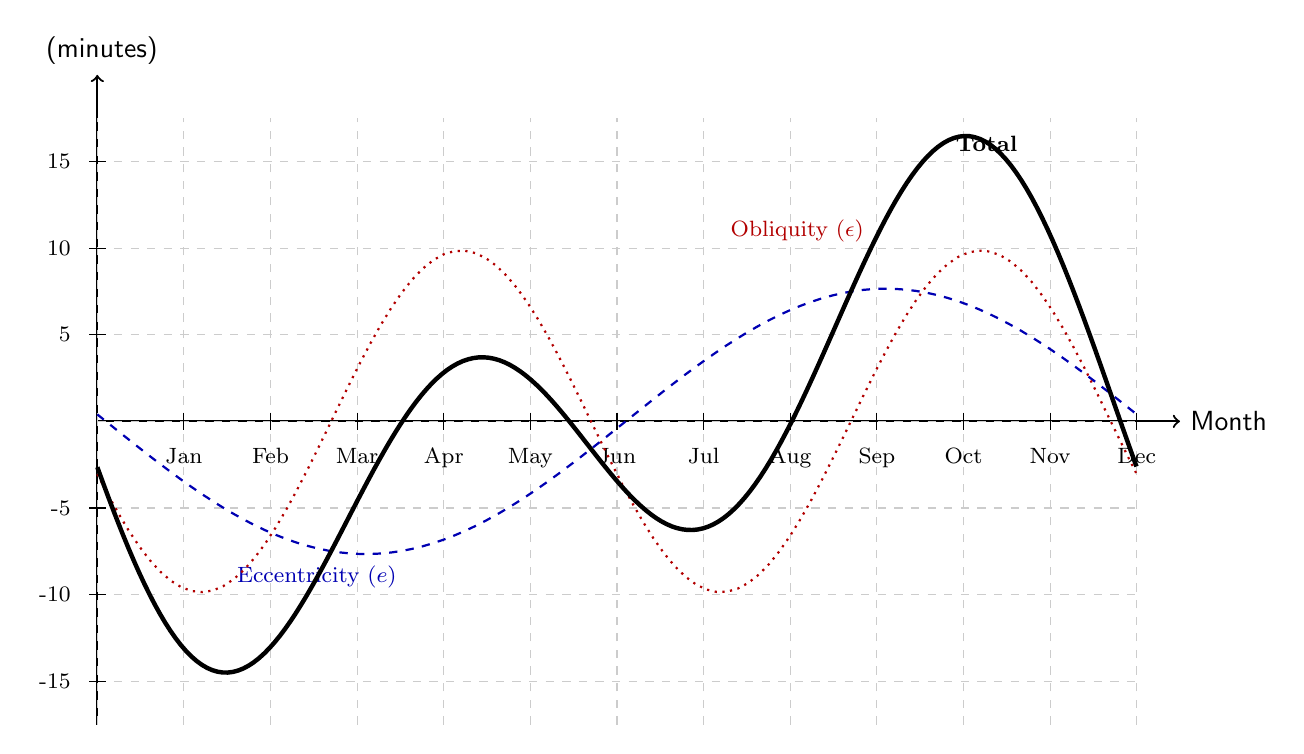
\begin{tikzpicture}[scale=1.1, font=\sffamily]
		\draw[->, thick] (0,0) -- (12.5,0) node[right] {Month};
		\draw[->, thick] (0,-3.5) -- (0,4.0) node[above] {$\EoT$ (minutes)};
		\draw[dashed, gray!40] (0,0) grid[xstep=1, ystep=1] (12,3.5);
		\draw[dashed, gray!40] (0,0) grid[xstep=1, ystep=1] (12,-3.5);
		
		% Ticks
		\foreach \x/\m in {1/Jan, 2/Feb, 3/Mar, 4/Apr, 5/May, 6/Jun, 7/Jul, 8/Aug, 9/Sep, 10/Oct, 11/Nov, 12/Dec} {
			\draw (\x, 0.1) -- (\x, -0.1) node[below=3pt, font=\footnotesize] {\m};
		}
		\foreach \y in {-15, -10, -5, 5, 10, 15} {
			\draw (0.1, \y*0.2) -- (-0.1, \y*0.2) node[left=3pt, font=\footnotesize] {\y};
		}
		
		% Component curves
		\draw[blue!70!black, thick, dashed, domain=0:12, samples=100] 
			plot (\x, {-7.66*sin(360*(\x-0.1)/12)*0.2});
		\node[blue!70!black, font=\footnotesize, right] at (1.5, -1.8) {Eccentricity ($e$)};
		
		\draw[red!70!black, thick, dotted, domain=0:12, samples=100] 
			plot (\x, {9.86*sin(720*(\x-2.7)/12)*0.2});
		\node[red!70!black, font=\footnotesize, right] at (7.2, 2.2) {Obliquity ($\epsilon$)};
		
		% Total curve
		\draw[black, ultra thick, domain=0:12, samples=200] 
			plot (\x, {(-7.66*sin(360*(\x-0.1)/12) + 9.86*sin(720*(\x-2.7)/12))*0.2});
		\node[black, font=\bfseries\footnotesize, right] at (9.8, 3.2) {Total $\EoT$};
	\end{tikzpicture}
	\caption{The Equation of Time decomposed into its two constituent physical components: orbital eccentricity ($e$, annual period) and obliquity ($\epsilon$, semi-annual period).}
	\label{fig:eot_decomposition}
\end{figure}

The total Equation of Time ranges between $-14.2\ \text{minutes}$ (in mid-February) and $+16.4\ \text{minutes}$ (in early November). Plotting the Sun's declination $\delta_\odot$ against the Equation of Time produces the famous figure-8 pattern known as the \emph{solar analemma}.

\section{Mean and Apparent Sidereal Time: The Equation of the Equinoxes}

Because the Earth is an oblate spheroid with an equatorial bulge, the gravitational forces exerted by the Moon and the Sun create torques that cause the Earth's rotation axis to precess and nutate in inertial space.

\begin{definition}[Mean versus True Equinox]
	\begin{itemize}
		\item The \emph{mean equinox} is the equinox position affected by smooth secular precession only.
		\item The \emph{true (apparent) equinox} is the instantaneous position of the equinox, including both secular precession and short-period nutation oscillations.
	\end{itemize}
\end{definition}

Sidereal time referenced to the mean equinox is \emph{Greenwich Mean Sidereal Time} ($\GMST$); sidereal time referenced to the true equinox is \emph{Greenwich Apparent Sidereal Time} ($\GAST$). They differ by the \emph{equation of the equinoxes}:
\begin{keyresult}
	\begin{equation}
		\GAST - \GMST = \Delta\psi\cos\epsilon \equiv \text{eqeq},
		\label{eq:equation_of_equinoxes}
	\end{equation}
\end{keyresult}
where $\Delta\psi$ is the nutation in longitude (dominated by the $18.6$-year regression of lunar nodes) and $\epsilon$ is the true obliquity. Because $|\text{eqeq}| \le 1.2\ \text{seconds}$, $\GMST$ suffices for casual observations, while $\GAST$ is essential for sub-arcsecond astrometry.

\subsection{Algorithmic Computation of GMST}

According to IAU conventions, $\GMST$ at $0^{\rm h}$ UT1 is computed from the Julian centuries $T$ elapsed since standard epoch J2000.0 ($T = (\JD - 2451545.0)/36525$):
\begin{equation}
	\GMST(0^{\rm h}\UT1) = 6^{\rm h}41^{\rm m}50.54841^{\rm s} + 8640184.812866^{\rm s}\,T + 0.093104^{\rm s}\,T^2 - 6.2 \times 10^{-6\,\rm s}\,T^3.
	\label{eq:gmst_iau_formula}
\end{equation}
At any instant of universal time $t_{\rm UT}$ (in hours):
\begin{equation}
	\GMST(t_{\rm UT}) = \GMST(0^{\rm h}\UT1) + 1.00273790935 \times t_{\rm UT}.
	\label{eq:gmst_instant}
\end{equation}

\section{Precession of the Equinoxes and Reference Epochs}

\begin{definition}[Lunisolar Precession]
	\emph{Lunisolar precession} is the slow, steady conical rotation of the Earth's spin axis around the normal to the ecliptic plane, with period $P_{\rm prec} \approx 25{,}772\ \text{years}$ (the Platonic Year). The spin axis traces out a cone of half-angle equal to the obliquity ($\epsilon \approx 23.44^\circ$), driven by the gravitational torque that the Sun and Moon exert on the Earth's oblate equatorial bulge --- the same torque-on-a-spinning-top mechanism responsible for ordinary gyroscopic precession.
\end{definition}

The vernal equinox drifts westward along the ecliptic at the rate:
\begin{equation}
	\dot\lambda_{\rm prec} \simeq 50.29''/\text{year} \approx 1^\circ/71.6\ \text{years}.
	\label{eq:precession_rate}
\end{equation}
Because the equatorial grid $(\alpha, \delta)$ is pinned to the moving equinox $\hat\gamma$, cataloged positions must always specify a standard epoch. The current international standard is epoch \textbf{J2000.0} (January 1, 2000, 12:00:00 TT).

To precess coordinates $(\alpha_0, \delta_0)$ from J2000.0 to an epoch $t$ with $\Delta t = t - 2000.0$ years:
\begin{keyresult}
	\begin{align}
		\alpha(t) &\approx \alpha_0 + (m + n\sin\alpha_0\tan\delta_0)\,\Delta t, \label{eq:precess_alpha} \\
		\delta(t) &\approx \delta_0 + (n\cos\alpha_0)\,\Delta t, \label{eq:precess_delta}
	\end{align}
\end{keyresult}
where the J2000.0 precession constants are $m = 3.075\ \text{s/yr} = 46.12''/\text{yr}$ and $n = 1.336\ \text{s/yr} = 20.04''/\text{yr}$.

\section{Modern Astronomical Time Scales: UT1, TAI, UTC, TT, and TDB}

Modern astrophysics requires a hierarchy of specialized time scales:

\begin{enumerate}
	\item \textbf{UT1 (Universal Time 1):} Measures the true rotation angle of the Earth about its axis, determined via VLBI observations of extragalactic quasars. Due to atmospheric winds, tidal friction, and core-mantle coupling, UT1 is non-uniform.
	\item \textbf{TAI (International Atomic Time):} A uniform atomic time scale generated by a weighted ensemble of hundreds of caesium-133 primary atomic clocks worldwide, defining the SI second ($9{,}192{,}631{,}770$ periods of the ground-state hyperfine transition).
	\item \textbf{UTC (Coordinated Universal Time):} The civil time standard. UTC runs at the SI rate of TAI, but integer \emph{leap seconds} are inserted at the end of June or December to maintain $|\UTC - \UT1| < 0.9\ \text{seconds}$:
	\begin{equation}
		\TAI - \UTC = \Delta\mathrm{AT} \quad (\text{currently } 37\ \text{seconds}).
	\end{equation}
	\item \textbf{TT (Terrestrial Time):} The theoretical coordinate time scale for clocks on the rotating geoid, free from Earth rotation irregularities:
	\begin{equation}
		\TT = \TAI + 32.184\ \text{s} \quad\Longrightarrow\quad \TT - \UTC = \Delta\mathrm{AT} + 32.184\ \text{s} \approx 69.184\ \text{s}.
	\end{equation}
	\item \textbf{TDB (Barycentric Dynamical Time):} The relativistic coordinate time scale evaluated at the Solar System Barycenter (SSB). It accounts for general relativistic gravitational redshift and orbital time dilation:
	\begin{equation}
		\TDB \approx \TT + 0.001657\sin(E + 0.01671\sin E)\ \text{s},
	\end{equation}
	where $E$ is the Earth's orbital eccentric anomaly. TDB is essential for pulsar timing arrays and interplanetary navigation.
\end{enumerate}

\section{Julian Date (JD) and Modified Julian Date (MJD)}

To track time continuously across millennia without calendar discontinuities, astronomers use the Julian Date system.

\begin{definition}[Julian Date]
	The \emph{Julian Date} ($\JD$) is the continuous count of days elapsed since Greenwich mean noon (12:00:00 UT) on January 1, 4713 BCE.
\end{definition}

\begin{definition}[Modified Julian Date]
	The \emph{Modified Julian Date} ($\MJD$) shifts the origin to Greenwich midnight and subtracts a large constant:
	\begin{keyresult}
		\begin{equation}
			\MJD \equiv \JD - 2{,}400{,}000.5.
			\label{eq:mjd_def}
		\end{equation}
	\end{keyresult}
	$\MJD = 0.0$ corresponds to midnight on November 17, 1858.
\end{definition}

\paragraph{Standard Astronomical Epochs:}
\begin{itemize}
	\item \textbf{Epoch J2000.0:} $\JD = 2{,}451{,}545.0$ (2000 Jan 1, 12:00:00 TT).
	\item \textbf{Epoch B1950.0:} $\JD = 2{,}433{,}282.423$.
\end{itemize}

\paragraph{Calendar Conversion Algorithm (Meeus 1998):}
For year $Y$, month $M$ ($1 \le M \le 12$), and decimal day $D$ (with UT fraction):
If $M = 1$ or $2$, set $Y \leftarrow Y - 1$ and $M \leftarrow M + 12$.
The Julian Date is computed via:
\begin{equation}
	A = \lfloor Y/100\rfloor, \qquad B = 2 - A + \lfloor A/4\rfloor,
\end{equation}
\begin{keyresult}
	\begin{equation}
		\JD = \lfloor 365.25(Y + 4716)\rfloor + \lfloor 30.6001(M + 1)\rfloor + D + B - 1524.5.
		\label{eq:jd_formula_meeus}
	\end{equation}
\end{keyresult}

With a continuous, unambiguous time coordinate now established, Chapter~2 turns to the companion problem of \emph{position}: fixing a coordinate grid on the celestial sphere itself. That grid is not static --- its very definition (the equatorial plane and the vernal equinox $\hat\gamma$) is tied to the precessing Earth axis derived above, which is why every catalogued equatorial coordinate must carry an epoch (Section~\ref{sec:coordinate_epochs}).
